\section{Portugal, Spain, the Netherlands and Luxembourg}\label{sec:cases}

\paragraph{Design.} The case study asks where output fluctuations are absorbed in four
countries. Each hypothesis was written down before any computation and follows from
definitions, from the accounting identity~\eqref{eq:identity} or from standard mechanisms.
Each makes predictions that can fail and that are evaluated by the same rule in the
comparison countries, so no prediction is tailored to one country. Three classes of
evidence are kept apart:
\begin{itemize}
  \item \emph{correlation}: cross-country associations with institutions;
  \item \emph{pattern consistent with a mechanism}: where output fluctuations are absorbed;
  \item \emph{identified causal effect}: none, because the designs of
    section~\ref{sec:identification} are uninformative.
\end{itemize}

\paragraph{Margins.} Each margin's response is the two-lag sum of its elasticity to GDP
growth, with 2020--2021 excluded. Intervals are 95\% synchronised circular block-bootstrap
intervals \citep{kunsch1989bootstrap}. By the identity, the elasticities of output per hour,
hours per worker and domestic employment sum to one.

\paragraph{Data.} The employment and hours data come from the national accounts
(\citetalias{eurostat_namq_10_pe}, \citetalias{eurostat_namq_10_a10_e}). Temporary and permanent employees
come from the Labour Force Survey (\citetalias{eurostat_lfsq_etgaed}, \citetalias{eurostat_lfsq_eegaed}), the
cross-country temporary and part-time shares from
\citetalias{eurostat_lfsq_etpga} and \citetalias{eurostat_lfsq_eppga}, and employment protection indicators from
the OECD \citep{oecd2020epl}. Eurostat publishes hours worked for Portugal but no
seasonally adjusted quarterly employment in persons, so its hours per worker and domestic
employment cannot be computed and two of its predictions cannot be evaluated. The protocol
had assumed wider coverage; its change log records the correction.

\paragraph{Overall result.} \val{cs_supported} of \val{cs_total} pre-registered predictions
is supported and \val{cs_contradicted} are contradicted; the rest are not determined
(table~\ref{tab:casestudy}). The cross-country correlations with institutions are a
separate, registered set of \val{cs_n_corr} correlations (subsection~\ref{sec:institutions}),
outside these \val{cs_total} predictions.

\subsection{Spain}

\paragraph{Association.} Spain's association is large and robust:
\begin{itemize}
  \item classical two-lag sum \val{cl_ES_excl} \val{cl_ES_excl_ci} for 2009--2026 without
    2020--2021;
  \item on the same 2009--2019 quarters, OLS gives \val{by_ES_ols} and the hierarchical
    model \val{by_ES} \val{by_ES_ci}; the gap is partly pooling and partly the common
    factor, which the hierarchical sum excludes;
  \item probability \val{claim_es_p} that its sum lies below the European mean, with the
    rule satisfied in \val{claim_es_holds} of \val{by_n_accepted} accepted fits.
\end{itemize}

\paragraph{Margins.} Spain absorbs output fluctuations almost entirely through
employment (figure~\ref{fig:margins}):
\begin{itemize}
  \item domestic-employment elasticity \val{cs_ES_e_dom} \val{cs_ES_e_dom_ci};
  \item output per hour \val{cs_ES_prod} \val{cs_ES_prod_ci}, an interval that includes
    zero.
\end{itemize}
\citet{bentolila2012twotier} attribute much of Spain's larger rise in unemployment in the
Great Recession, compared with France, to the gap between the dismissal costs of permanent
and temporary contracts. The pre-registered test that temporary employment is more
GDP-elastic than permanent employment gives \val{cs_p41es} \val{cs_p41es_ci} and is
\val{cs_p41es_verdict}. It is supported only in the \val{cs_p41es_settings} sensitivity
setting. The data therefore do not establish that temporary contracts carry Spain's
adjustment, and do not show that they cause it.

\subsection{Portugal}

\paragraph{Association.} Portugal's association is negative, but its significance depends
on the specification:
\begin{itemize}
  \item full sample: \val{cl_PT_full} \val{cl_PT_full_ci};
  \item without 2020--2021: \val{cl_PT_excl} \val{cl_PT_excl_ci};
  \item posterior median: \val{by_PT} \val{by_PT_ci}.
\end{itemize}
The Spain--Portugal difference \val{pair_ES_PT} the robustness set
(section~\ref{sec:heterogeneity}).

\paragraph{Margins.} Total hours respond to GDP almost as strongly in Portugal
(\val{cs_PT_h} \val{cs_PT_h_ci}) as in Spain (\val{cs_ES_h} \val{cs_ES_h_ci}). The
Spain--Portugal difference in the unemployment response \val{cs_pair_ES_PT_h} when
measured in hours worked.

\paragraph{Predictions.} The prediction that Portugal adjusts more through productivity
than Spain gives \val{cs_p52} \val{cs_p52_ci} and is \val{cs_p52_verdict}. The employment
comparison cannot be made with the published data.

\paragraph{A descriptive observation.} The following was not a registered prediction.
Participation rises with GDP in Portugal (\val{cs_PT_dp} \val{cs_PT_dp_ci} percentage
points per percent) but not in Spain. By identity~\eqref{eq:identity}, a labour force that
grows with output offsets part of the fall in unemployment that employment growth would
otherwise bring. With total hours responding alike in the two countries, this is one
accounting route to Portugal's smaller unemployment response. Whether it is the route
cannot be checked without quarterly employment in persons.

\subsection{The Netherlands}

\paragraph{Timing.} The posterior share of the Dutch response that comes from lagged GDP
growth is \val{by_NL_lagshare}. The registered rule for a delayed response holds in the
primary fit (probability \val{claim_nl_p}) but only in \val{claim_nl_holds} of
\val{by_n_accepted} accepted fits. Measured with four lags, the Dutch lagged share exceeds
Spain's by \val{cs_p31a} \val{cs_p31a_ci}, which is \val{cs_p31a_verdict} (supported only
in the \val{cs_p31a_settings} setting).

\paragraph{Margins.}
\begin{itemize}
  \item \emph{Output per hour:} the one supported prediction. Dutch output per hour is
    more GDP-elastic than Spanish, by \val{cs_p22} \val{cs_p22_ci} (Holm $p=$
    \val{cs_p22_holm}). A larger productivity response is a pattern consistent with labour
    hoarding, although hoarding cannot be separated from unmeasured effort or capacity
    utilisation.
  \item \emph{Hours per worker:} the difference from Spain, \val{cs_p21a} \val{cs_p21a_ci},
    is \val{cs_p21a_verdict}.
  \item \emph{Participation:} it responds less in the Netherlands than in Portugal
    (\val{cs_p23b} \val{cs_p23b_ci}, Holm $p=$ \val{cs_p23b_holm}), the opposite of the
    prediction, but this is not decided after adjustment.
\end{itemize}

\subsection{Luxembourg}

\paragraph{Association.}
\begin{itemize}
  \item \emph{Classical:} the sum is \val{cl_LU_verdict}: \val{cl_LU_full} on the full
    sample, \val{cl_LU_excl} without 2020--2021.
  \item \emph{Bayesian:} the posterior median is \val{by_LU} \val{by_LU_ci}.
  \item \emph{The weakness rule} requires the sum to lie above the European mean with
    probability at least $0.95$ and its 90\% interval to include zero. That probability is
    \val{claim_lu_p} in the primary fit, and the rule holds in \val{claim_lu_holds} of
    \val{by_n_accepted} accepted fits.
  \item \emph{The dynamic amendment.} In the two ARDL fits, which model the persistence
    the primary model misses, the rule \val{dyn_lu_ardl} on the long-run sum
    (probabilities \val{dyn_lu_ardl_p} and \val{dyn_lu_adf_p}). It holds because of
    Luxembourg's negative lagged-change coefficient, which shrinks its long-run multiplier;
    on the short-run sum the probability is \val{dyn_lu_adf_short_p}. These fits were
    registered as an amendment and are not part of the claim judgement, which keeps the
    original nine specifications.
\end{itemize}

\paragraph{Measurement.} GDP counts production by everyone working in Luxembourg, while
unemployment counts residents only, and cross-border commuters are a large share of
employment. If labour-input adjustment fell on commuters, domestic employment would respond
more than resident employment. It does not: the gap is \val{cs_p11} \val{cs_p11_ci}, and
both measures barely move with GDP:
\begin{itemize}
  \item domestic employment: \val{cs_LU_e_dom_pe} \val{cs_LU_e_dom_pe_ci};
  \item resident employment: \val{cs_LU_e_res} \val{cs_LU_e_res_ci}.
\end{itemize}
Instead, measured output per hour moves almost one for one with measured GDP
(\val{cs_LU_prod} \val{cs_LU_prod_ci}).

\paragraph{Two rival explanations, tested.} Output per hour is computed as the residual
$g-h$, where $h$ is the growth of hours. A weak link between output and labour input can
therefore come from the data as well as from the economy. A further registered study
(\texttt{GDP\_MEASUREMENT\_PROTOCOL.md}) tested two explanations with value added and
hours by industry \citepalias{eurostat_namq_10_a10}. Each test compares Luxembourg with
the median of the countries outside Luxembourg, Ireland and Malta.
\begin{itemize}
  \item \emph{Transitory noise in quarterly output.} If quarterly growth carried noise
    unrelated to labour input, measured growth would be negatively autocorrelated, and the
    correlation of hours with output would rise more than elsewhere once both are measured
    year on year, because aggregation averages the noise out. Luxembourg's growth
    autocorrelation is lower than the comparison group's (\val{gm_p11_lu_focus} against
    \val{gm_p11_lu_median}; Holm $p=$ \val{gm_p11_lu_holm}, \val{gm_p11_lu_verdict}). But
    its hours-output correlation does not rise at all: it is \val{gm_lu_c_q} quarter on
    quarter and \val{gm_lu_c_y} year on year, while it rises by a median
    \val{gm_p12_lu_median} elsewhere. That points away from noise, although it is not
    decided after adjustment (difference \val{gm_p12_lu} \val{gm_p12_lu_ci}, Holm
    $p=$ \val{gm_p12_lu_holm}).
  \item \emph{The financial sector.} Finance is \val{gm_lu_fin_va} of Luxembourg's value
    added and \val{gm_lu_fin_hours} of its hours; the next highest share of value added is
    about \val{gm_fin_va_next}. Yet removing finance from both output and hours barely
    changes the link. The hours elasticity changes by \val{gm_p21_lu_focus} and the Okun
    sum by \val{gm_p22_lu_focus} (verdicts: \val{gm_p21_lu_verdict} and
    \val{gm_p22_lu_verdict}).
    The output-per-hour elasticity is \val{gm_lu_prod} for all industries and
    \val{gm_lu_prod_n} outside finance.
\end{itemize}
By the interpretation rules fixed in that protocol, both explanations fail their tests,
and Luxembourg's weak output-labour link remains unexplained. Of
\val{gm_total} predictions, \val{gm_supported} is supported: Ireland's quarterly growth
is negatively autocorrelated (\val{gm_p11_ie_focus} against \val{gm_p11_ie_median}),
the signature of noise in its quarterly output. Its year-on-year correlation rises like
everyone else's, however, so the full signature is not established there either.
Ireland's modified domestic demand, published by its statistical office rather than
Eurostat, and sectoral composition beyond finance were not tested.

\subsection{Do the differences remain under other measures?}

\paragraph{Test.} If a difference between two countries reflects how much of their
labour-input adjustment falls on unemployment, it may disappear when labour input is
measured by employment or hours. Each pair whose unemployment responses differ was compared
again under resident employment, domestic employment and hours worked, where the data
exist. Of these pair-and-measure comparisons:
\begin{itemize}
  \item \val{cs_pairs_remain} remain;
  \item \val{cs_pairs_disappear} disappear;
  \item \val{cs_pairs_reverse} reverse.
\end{itemize}

\paragraph{By pair, in hours worked.}
\begin{itemize}
  \item Spain--Netherlands: \val{cs_pair_ES_NL_h};
  \item Spain--Luxembourg: \val{cs_pair_ES_LU_h};
  \item Spain--Portugal: \val{cs_pair_ES_PT_h};
  \item Netherlands--Luxembourg: \val{cs_pair_NL_LU_h}.
\end{itemize}

\subsection{Institutions}\label{sec:institutions}

The protocol predicted that stricter employment protection would weaken the unemployment
response. Spearman correlations across countries were computed with permutation $p$-values,
Holm-adjusted over six indicators in each of three variants. Of the \val{cs_n_corr}
correlations, \val{cs_n_corr_contra} point the other way at the registered level:
\begin{itemize}
  \item regular-contract protection against the classical sum: $\rho=$
    \val{cs_eplr_cl_rho} over \val{cs_eplr_cl_n} countries (Holm $p=$
    \val{cs_eplr_cl_holm});
  \item temporary-contract protection against the Bayesian sum without Luxembourg and
    Ireland: $\rho=$ \val{cs_eplt_noluie_rho} over \val{cs_eplt_noluie_n} countries (Holm
    $p=$ \val{cs_eplt_noluie_holm}).
\end{itemize}
With all twenty countries the second correlation is \val{cs_eplt_by_rho} (Holm $p=$
\val{cs_eplt_by_holm}). These are correlations among at most twenty countries, measured
once in 2008. They contradict the predicted direction, but they say nothing about what
employment protection does.

\subsection{Comparison with the earlier claims}

Table~\ref{tab:claims} sets the earlier analysis's three descriptive claims, and the two
explanations we tested of the kind it suggested, against the evidence. No claim about Portugal was documented, so none
is assessed. Several explanations could not be
tested reliably, and the protocol said so before any result:
\begin{itemize}
  \item the 2012 labour-market reforms in Spain and Portugal, which coincide with the
    sovereign-debt crisis;
  \item short-time work, for which no harmonised quarterly take-up data exist before 2020;
  \item collective bargaining, minimum wages and benefit generosity;
  \item sectoral composition.
\end{itemize}

\begin{table}[t]\centering\small
\caption{The earlier claims against the evidence. ``Supported'': the evidence agrees under
every accepted specification. ``Qualified'': part of the claim holds, or it holds only
under some specifications. ``Contradicted'': the evidence points the other way at the
registered level. None of these verdicts is causal.}\label{tab:claims}
\begin{tabular}{p{0.2\textwidth}p{0.5\textwidth}p{0.2\textwidth}}
\toprule
Claim & Evidence & Verdict \\
\midrule
Spain: large association
  & Below the European mean with probability \val{claim_es_p}; rule holds in
    \val{claim_es_holds} of \val{by_n_accepted} accepted fits. Adjustment runs through
    employment (\val{cs_ES_e_dom}).
  & Supported \\
\addlinespace
Netherlands: delayed response
  & Lag share \val{by_NL_lagshare}; rule holds in \val{claim_nl_holds} of
    \val{by_n_accepted} fits. Lag share against Spain \val{cs_p31a_verdict}. Output per hour
    absorbs more than in Spain (Holm $p=$ \val{cs_p22_holm}).
  & Qualified \\
\addlinespace
Luxembourg: weak association
  & Classical sum \val{cl_LU_verdict}; Bayesian rule holds in \val{claim_lu_holds} of
    \val{by_n_accepted} registered fits, but \val{dyn_lu_adf} on the long-run sum in both
    ARDL amendment fits.
  & Qualified \\
\addlinespace
Explanation: the commuter mismatch
  & Domestic-minus-resident gap \val{cs_p11} \val{cs_p11_ci}. The two rival explanations
    tested afterwards, transitory noise in quarterly output and the financial sector, fail
    their tests too.
  & Not supported \\
\addlinespace
Explanation: employment protection weakens the response
  & \val{cs_n_corr_contra} of \val{cs_n_corr} registered correlations have the opposite
    sign at the registered level (\val{cs_eplr_cl_rho}, \val{cs_eplt_noluie_rho}); the
    rest are not determined.
  & Contradicted (correlation only) \\
\bottomrule
\end{tabular}
\end{table}

% Generated by eu-okun publication. Do not edit.
\begin{table}[t]\centering\small
\caption{Pre-registered predictions of the case study (two-lag elasticities to GDP growth, 2020--2021 excluded; block-bootstrap 95\% intervals; Holm adjustment over the determinable predictions). A supported prediction is a pattern consistent with a mechanism, not a causal effect.}
\label{tab:casestudy}
\footnotesize
\begin{tabular}{llrrl}
\toprule
Prediction & Statistic & Estimate [95\%] & Holm $p$ & Verdict \\
\midrule
P1.1 & \texttt{beta\_e\_dom\_pe(LU) - beta\_e\_res(LU)} & $+0.01$ $[-0.05, +0.05]$ & $1.000$ & not determined \\
P1.3 & \texttt{gap(LU) - median gap(others)} & $+0.00$ $[-0.06, +0.05]$ & $1.000$ & not determined \\
P2.1a & \texttt{beta\_hpw(NL) - beta\_hpw(ES)} & $-0.08$ $[-0.60, +0.23]$ & $1.000$ & not determined \\
P2.1b & \texttt{beta\_hpw(NL) - beta\_hpw(PT)} & n/a & n/a & not determined \\
P2.2 & \texttt{beta\_prod(NL) - beta\_prod(ES)} & $+0.73$ $[+0.31, +1.23]$ & $0.022$ & supported \\
P2.3a & \texttt{beta\_dp(NL) - beta\_dp(ES)} & $-0.01$ $[-0.15, +0.15]$ & $1.000$ & not determined \\
P2.3b & \texttt{beta\_dp(NL) - beta\_dp(PT)} & $-0.22$ $[-0.39, -0.06]$ & $0.100$ & not determined \\
P3.1a & \texttt{share(NL) - share(ES)} & $+0.46$ $[-0.13, +1.04]$ & $1.000$ & not determined \\
P3.1b & \texttt{share(NL) - share(PT)} & n/a & n/a & not determined \\
P4.1 ES & \texttt{beta\_temp(ES) - beta\_perm(ES)} & $+0.72$ $[-1.28, +2.08]$ & $1.000$ & not determined \\
P4.1 PT & \texttt{beta\_temp(PT) - beta\_perm(PT)} & $+0.10$ $[-1.51, +1.16]$ & $1.000$ & not determined \\
P4.1 NL & \texttt{beta\_temp(NL) - beta\_perm(NL)} & $-0.46$ $[-2.07, +1.06]$ & $1.000$ & not determined \\
P5.1 & \texttt{beta\_e\_dom(ES) - beta\_e\_dom(PT)} & n/a & n/a & not determined \\
P5.2 & \texttt{beta\_prod(PT) - beta\_prod(ES)} & $-0.06$ $[-0.51, +0.28]$ & $1.000$ & not determined \\
\bottomrule
\end{tabular}
\end{table}


\begin{figure}[t]\centering
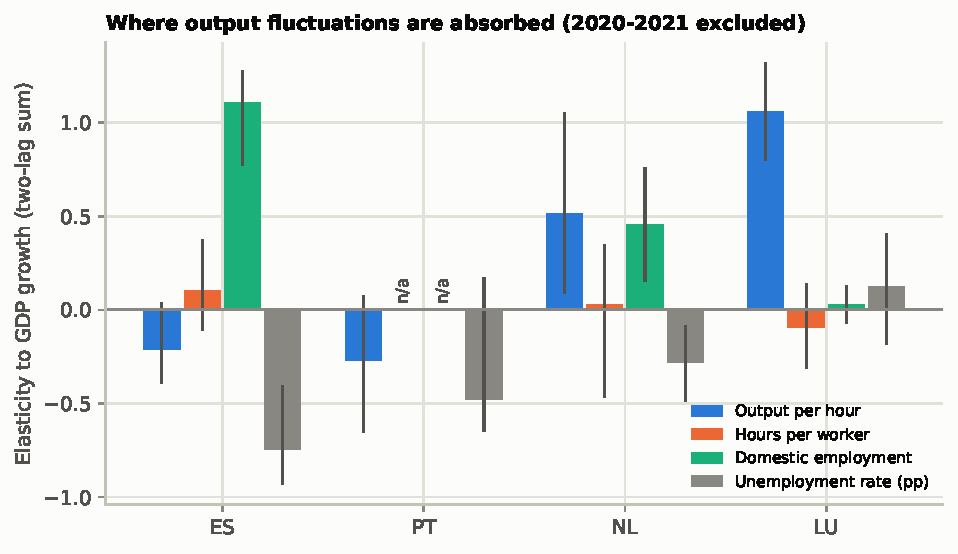
\includegraphics[width=0.8\textwidth]{fig6_margins.pdf}
\caption{Elasticities to GDP growth of output per hour, hours per worker, domestic
employment and the unemployment rate (two-lag sums, 2020--2021 excluded, 95\%
block-bootstrap intervals). Eurostat publishes no seasonally adjusted quarterly employment
in persons for Portugal, so its hours per worker and domestic employment are not
available. Portugal's unemployment elasticity, \val{cs_PT_du} \val{cs_PT_du_ci}, has a
bootstrap interval that crosses zero, while the HAC interval of table~\ref{tab:countries}
(\val{cl_PT_excl} \val{cl_PT_excl_ci}) does not. The point estimates agree; the
percentile interval of the block bootstrap is wide and asymmetric, which suggests a few
influential quarters, whereas the HAC interval relies on normal critical
values.}\label{fig:margins}
\end{figure}
